
\documentclass[a4paper,doc, natbib]{apa6} %apa6/jou/man/doc

\usepackage[english]{babel}
\usepackage[utf8x]{inputenc}
\usepackage{amsmath,amssymb}
\usepackage{graphicx}
\usepackage[colorinlistoftodos]{todonotes}

\usepackage{multicol}
\usepackage{multirow}
\usepackage{booktabs} %booktabs package makes nice tables!
\usepackage{url}
\usepackage{rotating}
\usepackage[toc,page]{appendix}
\usepackage{color}
\usepackage{subscript}
\usepackage{threeparttable}
\usepackage{threeparttablex}
\usepackage{longtable}
\usepackage{times}
\usepackage{lipsum}

\title{Paper needs a title}
\shorttitle{Paper needs a subtitle}

\author{Janine Hoffart\\Jana Jarecki\\Jörg Rieskamp}
\affiliation{University of Basel}

\leftheader{XXXXXXXXXXXXXXXXX,XXXXXXXXXXXXXXXXXXXXX,XXXXXXXXXXXXXX}

\abstract{
\lipsum[1]
}
\keywords{Affect heuristic, risk--return belief, stock market}

\authornote{%This research is supported by a grant (SNF \# 143854) of the Swiss National Science Foundation to the second and third author.

%Correspondence concerning this article should be addressed to Janine Christin Hoffart. University of Basel, Department of Psychology, Missionsstrasse 62a, 4055 Basel, Switzerland.  E-mail: janine.hoffart@unibas.ch
}

\begin{document}
\maketitle

ADD QUOTES (From our studies)

The two quotes above symbolize how risk can have many faces. Indeed, the concept of risk does not have a universally accepted definition (XXX). While in Finance risk is often defined as variance or semi-variance of returns \citep{Markowitz1952, Markowitz1991, Markowitz1959}, people do not necessarily understand the concept of risk as volatility \citep{Mohr2010a}. Instead, people often relate to loss potential when they think about riskiness \citep{Duxbury2004, Sachse2012}. This mismatch in definitions can have dramatic consequences. For instance, consider a financial institution provides information about the riskiness of an asset, where risk is defined a volatility. A potential buyer retrieves this information to make a buy or sell decision. Importantly, she does not understand risk as volatility but as probability of a loss or severity of a loss. In this scenario, the buyer's subjective perception of the asset's performance might dramatically differ from the objective performance of the asset. This is because buyers due to their different understanding of the risk concept interpret the provided information differently (schlecht geschrieben, drüber lesen und präziser sein). Although constructed, the scenario above is realistic: Figure \ref{fig:pfrisk} displays how a large Swiss bank communicates risk information about funds to their clients. They graphically describe the riskiness of the asset on a scale from very low to very high. Dramatically, they only define how they conceptualize risk (i.e., as volatility) in a separate document. 
% https://www.postfinance.ch/pfch-web/feed-direct/postfinance/vfund/CH0006869207_en.pdf?method=pdf&isin=CH0006869207&lang=en

% https://www.postfinance.ch/en/private/products/investing-trading/fund-range.html/feed/fragment/postfinance/fragment2016/funds/fundDetail.jsp?valor=686920&market=393&currency=CHF 
% retrieved 5.9.2017; 16:58

Here, we aim to understand people's concept of \textit{risk} and how volatility should be communicated in order for people to understand it accurately. To do so, in two studies, we assessed people's perceived volatility of returns in situations of full information and uncertainty using various questions. Further, we assessed how well people's judgments of variance and return resembled the objective risk--return trade--off. 
(Affect heuristic einbringen)

\begin{figure}[!htbp] 
  \centering
 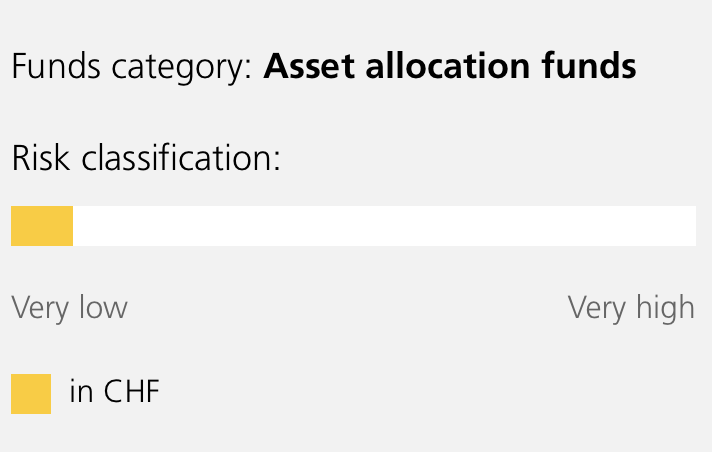
\includegraphics[width=.4\linewidth, keepaspectratio]{pf_risk1.png} 
  \caption{}
  \label{fig:pfrisk}
\end{figure}
%\section{Definitions of risk}

\section{Risk--Return trade--off}
In life, larger returns are often associated with larger risks. \texit{Return} usually describes the expected outcome value of an option and \textit{risk} relates to the variance of possible outcomes. The concept of a positive correlation between risk and returns is fundamental to finance and forms the basis of \citeauthor{Markowitz1952}'s (\citeyear{Markowitz1952}) mean variance model. The model assumes that investors face trade-offs between the expected returns of investments and the variance of returns. To date, risk--return models have been applied widely \citep[e.g.,][]{Weber2008, Mohr2010a} and shown to predict behavioural as well as neural data \citep{Mohr2010a}. \cite{Sunden1998} have reported that people understand the risk--return trade--off and use it to inform investment decisions.


Contrarily to the widely accepted notion that risks and returns are positively correlated (but see for a challenge of this notion CITATION), people often seem to neglect this regularity when judging risks and expected returns of options. Often, they judge options with larger returns as less risky than options with lower returns (CITATIONS). One common explanation for this finding is that people heuristically use their affective attitudes towards options to infer risks and returns (CITATION). As a consequence, options that trigger positive affects are perceived as less risky and more profitable than options that trigger negative affects (CITATION). 

\subsection{The affect heuristic and people's perception of risks and returns}
Several studies have suggested that people systematically believe that larger returns are associated with lower risks than smaller returns \citep[e.g.][]{Shefrin2001}. This belief contradicts the objective relationship between risks and returns. Cognitive biases have been proposed as explanation for the mismatch between people's assumption of a negative risk--return correlation and the objective positive risk--return correlation. \cite{Shefrin2001} has proposed the representative heuristic as explanation for people's biased risk--return representation. He argued that people judge companies with regards to how \textit{good} they are. If a company is perceived as a \textit{good} company, it's stocks will be associated with high future returns and safety. \cite{Kempf2014} have experimentally shown that people's affective attitude towards companies indeed predict how people judge the risks and future returns of these companies. Positive affective attitudes towards companies were related to low risk judgments and high return judgments. Negative affective attitudes on the other hand were related with high risk judgments and low return judgments. 

\subsubsection{Definition and Measures of Risk}
In most studies that investigated people's risk and return assumptions, participants were asked to judge as how risky they perceive a stock (XXX). Importantly, several papers suggest that no unique concept of risk exists (XXX).

\subsubsection{Objective definition of risk in Finance}
%Risk is a fundamental concept of many financial theories.
Depending on the theory, even in Finance, risk has different definitions. In his early work, \cite{Markowitz1952}% suggested that risk is an important factor for portfolio selection. He 
suggested that the variance of returns can be used as proxy for the commonly used term risk. Slightly later, he argued that not variance but semi-variance may be better suited to conceptualize risk \citep{Markowitz1959}. This is because semi-variance is only concerned with variance below a threshold as for instance the average return or zero. Hence, semi-variance describes the proportion of variance that is adverse for investors \citep{Markowitz1991}. However, not all definitions of risk commonly used in Finance relate to variance and semi-variance. Other definitions include standard deviation of returns, expected value of loss, expected absolute deviation, probability of loss and maximum loss (CITATIONS).
While risk already has several meanings in the financial literature, 
\subsection{Subjective use of the term risk}
The 



%

 While in finance, risk clearly is associated to variance, in everyday life, risks are often associated to losses (XX). Given this variation in the definition of risk, the question raises what exactly people respond to when they are asked to judge the riskiness of a stock. On the one hand, people's judgments might related to \textit{variance}, on the other hand, people's responses might relate to \textit{potential losses}. To more clearly investigate whether the affect heuristic holds when people clearly respond to variance, we conducted two studies. In Study 1, we aim to identify which is the best construct to measure risk--as--variance. To do so, we ask people to judge graphs stock returns with various scales. XX of these scales are related to variance questions (XXX) and XXX of the scales are related to loss questions (XX). We argue that if we aim to measure people's perception of risk--as--variance, we need to use a scale that clearly means risk--as--variance across people. In Study 2, we replicate previous studies on the affect heuristic. In this study, we ask people to judge XXX on two scales. Those scales are first risk and second the scale that has proven to measure risk--as--variance best in Study 1. We also assess people's affective attitude towards XXX to understand whether the affect herustic still holds when we clearly ask a question that measures people's variance beliefs. 

While some of the definitions describes above, relate to how people use term risk to communicate, others do not. Generally, 

Often, there risk is defined as volatility of returns. However, other 

Kights used to communicate probabilities
- objective
- subjective

\section{}


a.)	Risk & return: correlation in life
b.)	Risk & return: How people think about correlation
-	examples
c.)	Explanation for diverging findings
-	Affect heuristic
d.)	Problems with risk questions
e.)	Our approach
f.)	Results
g.)	Replicate affect heuristic with (1) original question (2) new question
	Is affect heuristic robust?
	Is it moderated by the question that is used?












%Recently, also psychologists have started to show interest in the systematic relationship between risks and return. Special interest has been dedicated to studying whether people exploit the risk--return taxonomy to inform decisions. \cite{Weber2005} have demonstrated that, in an experimental setting, participants used information about asset type (i.e., bond vs. stock) to judge expected returns and risks: Bonds were judged as less risky at the costs of lower expected returns. More recently \cite{Pleskac2014} have conducted a large scale analysis of real life risky decision options in every day environments. They found evidence for a positive correlation between risk and return in many domains of real life. Furthermore, they experimentally showed that participants assume a correlation between risk and return when they make probability judgments under uncertainty. 


authors do not give definitions for risk and benefit. Make claims that risks and benefits would show a certain correlation and state this as facts. But do not
\section{Methods}
\subsection{Participants}
We recruited 103 (41 female, 62 male) people residing in Germany via ClickWorker, an online crowd-sourcing platform. 
Before we analysed the data, we excluded the data of $3$ people ($1$ female, $2$ male) who indicated that they did not pay attention during the Study. We further excluded the data of $1$ man who indicated that he did not understand the instructions. Furthermore, we excluded three men who gave the same response to all stimuli for at least one response scale. %We did non know whether these people only clicked thrugh or were serious. 


The remaining $96$ people were on average $37$ years old ($SD_{age} = 12.2$; $range_{age}: 18 -- 65$). Most people's ($90$) native language was german, the remaining $6$ people did not specify their native language (Haben OTHER angegeben, das heisst native langugae war nicht im choice set. Naeher beschreiben?!). All participants had a school degree, $37$ people went to University and had at least a Bachelor's degree. 
The study was approved by the ethical committee of the University of Basel. People gave informed consent and were reimbursed for their participation (4.5 Euro roughly \$ 4.83 at the time of the Study).

\subsection{Materials and Procedure}
To create the stimuli, we retrieved a list of the twenty most traded stocks of Switzerland on October 27th 2016 (See Appendix). Then, we downloaded the daily start and end share prices of those stocks for January 2001 until December 2015. For one stock (Julius Baer) we only had data starting from 2009. We therefore excluded this stock from the stimulus set. For the remaining 19 stocks, we calculated the yearly return of investment and graphically displayed it in $\%$ (See Figure XXX for an overview of the stimuli that we used). Importantly, we did not indicate to which Company individual graphs related. 

We presented the 19 stocks repeatedly in eight blocks in which we asked our participants to rate the graphs. Within blocks, we randomised the order of presentation of stocks and repeatedly asked the same question for each stock (Table \ref{table:Questions}). Between subjects, we randomised the order of blocks. Generally, we asked three questions dealing with \textit{variability} of returns, one question dealing with \textit{risk} of that stock, three question dealing with \textit{losses}, and one question dealing with \textit{returns} in general. 


\begin{table}
\centering
\begin{threeparttable}
\caption{Overview of questions}
\small
\label{table:Questions}
\begin{tabular} {lll}
\toprule
Scale & Question & Format  \\
&&&
\multirow{1}{*}{Risk} & How risky do you judge the stock? & 7--point Likert \\
\midrule
\multirow{3}{*}{Variability} & How large do you judge the variability (variance) of the stock? & 7--point Likert\\
&  How large do you judge the average fluctuation of the stock returns? & 7--point Likert\\ 
 & How predictable do you judge the  stock (measured from 2003)? & 7--point Likert\\
\midrule
\multirow{4}{*}{Loss} & How large do you judge the expected average loss of this stock? &  $\%$ points \\
     & How large do you judge the average loss of this stock? & $\%$ points\\
     & How large do you judge the probability of making a loss with this stock & $\%$ points\\
     &  in a randomly selected year? & \\
\midrule

\multirow{1}{*}{Return} & How large do you judge the average return of this stock? & 7--point Likert \\
\bottomrule
\\
\end{tabular}
\begin{tablenotes}
\small
\item
 \textit{Note}. Overview about the different questions with which we assessed the stocks. All Likert scales besides the \textit{return} scale were unipolar. The \textit{return} scale was biploar ranging from extremely large lossed to extremely large gains.

\end{tablenotes}
\end{threeparttable}
\end{table}















\subsubsection{Coding open ended question}
\begin{itemize}
\item Three people coded the responses individually, 
\item Deductive categories
\item 
\item 
\end{itemize}

\section{Results}
For all following analyses of this manuscript we used the software R \citep{R2014}. 
\subsection{Which scale measures objective variance best?}
First, we analyzed how well responses to the different variance scales measure objective variance. Figure \ref{fig:rsvo} illustrates people's responses to the different response scales as function of objective variances of returns. Higher objective variance was positively correlated with larger perceived fluctuation ($r_{s} = .72, p < .05$); larger perceived variation ($r_{s} = .69, p < .05$) and larger perceived risk ($r_{s} = .49, p < .05$). It was negatively correlated with perceived predictability ($r_{s} = -.55, p < .05$). We ran separate ordinal regressions for each scale with objective variance as predictor and participants id as random effect. Table X shows the coefficients of the regression.

(Table \ref{table:QrdReg1}).




\begin{table}
\centering
\begin{threeparttable}
\caption{XXX}
\small
\label{table:QrdReg1}
\begin{tabular} {llll}
\toprule
Scale & Mean coefficient (SE) & Variance (SE) & Log Likelihood\\
& Objective risk& Random effect of participants&&
&&&&
\multirow{1}{*}{Fluctuation} &$24.32$ ($.85$)&  $1.01$ ($1.01$) & $-2656$ \\
\multirow{1}{*}{Variability} &$21.98$ ($.8$)&  $.51$ ($.71$) & $-2754$ \\
\multirow{1}{*}{Predictability} &$14.6$ ($.66$)&  $.76$ ($.87$) & $-3041$ \\
\multirow{1}{*}{Risk} &     $12.54$ ($.63$)        &  $1.15$ ($1.07$) & $-3007$ \\
\bottomrule
\\
\end{tabular}
\begin{tablenotes}
\small
\item
 \textit{Note}. Results ordinal regression.

\end{tablenotes}
\end{threeparttable}
\end{table}



Next, we repeated the correlation analysis for individual participants. Two people's responses were excluded from this analysis because their responses on at least one scale did not differ between stimuli. Figure \ref{fig:rsvoind} displays correlation coefficients between the objective variance of returns and people's responses to the different responses scales separately per participant. The graph reveals that correlation coefficients for the fluctuation question are most often (XXX of 97 participants) and most strong positively correlated with objective variance. 

\begin{itemize}
\item Compare sizes of correlation coefficients
\item 
\item 
\end{itemize}


\begin{figure}[!htbp] 
  \centering
 \fitfigure[]{risksub_varobj.pdf} 
  \caption{Objective variance of the returns (y--axis) as function of responses on the different scales (x--axis). The dots display individual responses; the dot-size response frequencies.}
  \label{fig:rsvo}
\end{figure}


\begin{figure}[!htbp] 
  \centering
 \fitfigure[]{risksub_varobj_ind.pdf} 
  \caption{Correlation coefficient (y--axis) for individual participants between objective variance of the returns and responses on different scales (main). The colour of the dots indicate whether the correlation coefficient reached significance (black) based on $p < .05 / (97 * 4)$ or not (grey)}
  \label{fig:rsvoind}
\end{figure}


\subsection{Does risk scale measure anything beyond variance?}
As Figure \ref{fig:rsvo} illustrates, the question how risky people perceive the stock based on the shown returns correlates positively with objective variance of the returns. However, the size of the correlation coefficient between responses on the risk scale and objective variance is the lowest of all coefficients. To analyse whether the risk scale measures anything beyond variance, we analyzed the responses to the open question at the end of the questionnaire. There, we asked people what they relate to high risk of a stock. XX
Next, we correlated people's responses on the risk scale with several objective risk measures. Figure XXXXXX displays the results. The Figure indicates that the correlation between subjective risk perception and objective variance is similarly high as the correlation between subjective risk perception and XXXXX. However, also fluctuatuion and objective risk scales are correlated. This is the case because objective measures show correlation: Loss and variance. To account for this correlation, we calculated correlation between subsets of stimuli where variance and loss are not correlated. We did this by repeatedly (10'000 times) sampling responses to 3,4,5,6,7,8 stimuli. Then - which correlation is below $r = .01$. 



To better understand where on the dimensions \textit{variance} and \textit{loss} the question about risk can be located, we conducted a factor analysis. 

\begin{itemize}
\item risk subj. has lowest correlation with obj. variance
\item analyse questions --> indicate that risk is also related to loss
\item risk subj. correlation with several objective risk measures --> similarly high correlation between some loss measures and risk
\item factor analysis
\end{itemize}


\subsection{Do people correctly report risk return correlation?}
\begin{itemize}
\item objective correlation is positive
\item people report positive correlation when asked for fluctuation & variability
\item people report negative correlation when asked for fluctuation & variability
\item can this be explained because some people talk about somethig loss related? repeat analysis only based on ppl who do not mention losses in open ended questionnaire
\item factor analysis

\end{itemize}


\section{Experiment 2}
\subsection{Methods}
We recruit people on Clickworker. 

\subsection{Results}

\subsubsection{Risk--Return estimates}
We analyzed people's responses to the variance questions and the return question. First, we investigated whether people's responses to the risk question matched objective variance. Figure \ref{fig:rsvoS2} shows people's responses split by risk question (risk vs. risk (as variance) vs. fluctuation) and graph condition (Graph seen yes vs. no). For all six cases, people's judgments were positively correlated with objective variance. The Spearman correlation coefficients ranged from .19 to .72.
\begin{figure}[!htbp] 
  \centering
 \fitfigure[]{risk_objsubj_Study2.pdf} 
  \caption{Responses to the variance questions (y--axis) as function of objective variance of the returns (x--axis). The title and the y--axis label describe the variance questions that were asked. The dots display individual responses; the dot-size response frequencies. The upper (lower) row displays responses in the graph (no graph) condition. }
  \label{fig:rsvoS2}
\end{figure}
To examine how well objective variance predicts people's responses to the variance questions, we calculated ordinal regressions where we predicted people's responses as function of objective variance and random participant effects separately for each question and split out by graph condition. Objective variance predicted responses to the fluctuation question best both in the graph ($\beta$ = .18, AIC = 2157) as well as the no graph ($\beta$ = .05, AIC = 2633) condition ($\beta$_{Risk (measured as variance; graph)} = .1, AIC_{Risk (measured as variance; graph)} = 2538, $\beta$_{Risk (measured as variance; no graph)} = .03, AIC_{Risk (measured as variance; no graph)} = 2684, 
$\beta$_{Risk; graph} = .08, AIC_{Risk; graph} = 2501, $\beta$_{Risk; no graph)} = .04, AIC_{Risk; no graph)} = 2848)


Next, we investigated how people's responses to the return question matched objective variance. Figure \ref{fig:retsvoS2} shows people's responses split by variance question (risk vs. risk (as variance) vs. fluctuation) and graph group (Figure seen yes vs. no). In the graph condition, people's judgments were positively correlated with objective returns. However, in the no--graph condition, people's judgments were negatively correlated with objective returns. Interestingly, a comparison of the AICs of the ordinal regressions reveal that people




\begin{figure}[!htbp] 
  \centering
 \fitfigure[]{ret_objsubj_Study2.pdf} 
  \caption{Responses to the return questions (y--axis) as function of objective variance of the returns (x--axis). The title describe the variance questions that were asked. The dots display individual responses; the dot-size response frequencies. The upper (lower) row displays responses in the graph (no graph) condition. }
  \label{fig:retsvoS2}
\end{figure}


Table XXX shows response frequencies to the \textit{risk} question split by the question that we asked and whether people have seen the graph. 



\subsubsection{Affect}
People's affective ratings were generally XXX. Across countries, xx (\%) of people's responses were above three, i.e. better than the mean (\texit{good -- bad} scale: xx (\%), \texit{interesting -- boring} scale: xx (\%), \texit{strong -- weak} scale: xx (\%), \texit{active -- passive} scale: xx (\%)). We compared people's response frequencies to the affective rating scales with a Chi square test (XXXX Hoffentlich nicht. Falls nicht. We cannot reject the null hypothesis, suggesting that generally, people's affective attitude towards the countries does not differ beteen conditions. ).
Figure XXX displays people's affective ratings split by company and scale (rows). Table XXX shows how responses to the different scales were correlated. The correlation coefficiens are XXX and range from XX to YYY. Cronbachs $\alpha$ is XXX which indicated that.... Given that the responses for all scales are correlated and Cronbachs $\alpha$ is high, for every individual participant (j), we calculate thh mean rating on all scales per country (i). We will use this aggregate variable that describes people affective attitude towards countries (AA\subscript{j,i}) for further analysis. \textcolor{red}{(Noch PCA rechnen um zu gucken, ob equal weighting richtig ist? Oder vielleicht alle Skalen drin lassen?).}


\section{Discussion}

\bibliography{refJanine}
\end{document}
